\chapter{Ergebnisse}\label{chap:ergebnisse}
\section{Genauigkeit bei 768 Trainingsfällen}
Tabelle~\ref{tab:fehler} und Abbildung~\ref{fig:genauigkeit} zeigen den vollständigen Feldfehler für die ausgewählten Familienkonfigurationen. Mittelwert und P95 werden je Lauf über Fälle bestimmt und für neuronale Modelle anschließend über drei Initialisierungen gemittelt. Das Maximum ist das größte tatsächlich beobachtete Fallmaximum über die jeweiligen Läufe. Für POD--GPR liegt ein deterministischer Vollpool-Hauptlauf vor; seine zwei zusätzlichen Fits sind Zeitwiederholungen, keine unabhängigen Datenziehungen.
\begin{table}[htbp]\centering\caption{Gewichteter relativer Feldfehler bei $N=768$. Angaben in Prozent.}\label{tab:fehler}
\small\begin{tabular}{lrrr rrr}\toprule
& \multicolumn{3}{c}{Interpolation} & \multicolumn{3}{c}{Extrapolation}\\
\cmidrule(lr){2-4}\cmidrule(lr){5-7} Methode & Mittel & P95 & Max. & Mittel & P95 & Max.\\\midrule
MLP & 4,64 & 14,78 & 58,59 & 16,24 & 50,74 & 638,23\\
RBF & 7,41 & 22,57 & 97,21 & 32,67 & 102,03 & 1253,55\\
POD--MLP & 4,78 & 15,73 & 43,78 & 13,74 & 47,82 & 286,56\\
POD--GPR & 0,55 & 2,20 & 6,65 & 3,85 & 15,85 & 88,55\\\bottomrule\end{tabular}\end{table}
\begin{figure}[htbp]\centering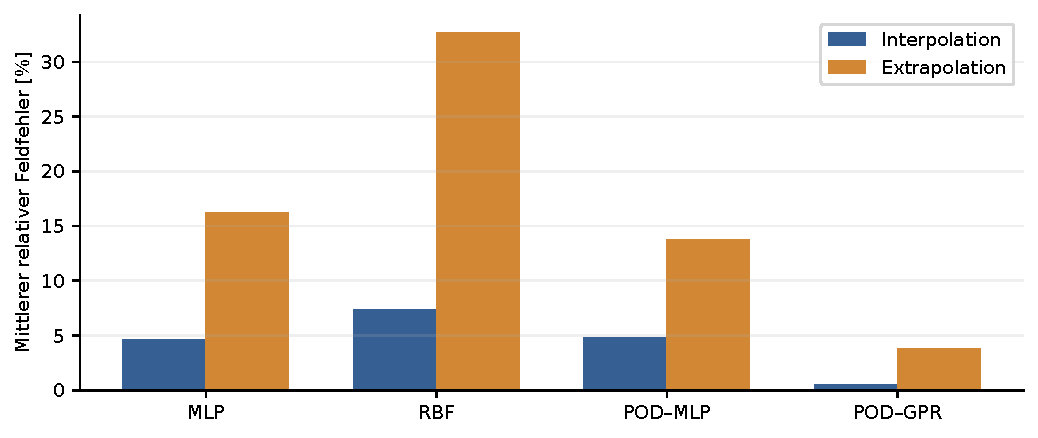
\includegraphics[width=.88\textwidth]{genauigkeit.pdf}\caption{Mittlerer relativer Feldfehler bei $N=768$. Neuronale Werte sind Mittel über drei Initialisierungen; POD--GPR umfasst einen Hauptlauf. Eigene Darstellung der Studienergebnisse.}\label{fig:genauigkeit}\end{figure}
POD--GPR erzielt auf beiden untersuchten Testverteilungen den kleinsten mittleren Fehler. Der Unterschied zwischen Interpolations- und Extrapolationsfällen ist bei allen Methoden deutlich. Auch für POD--GPR liegt das beobachtete Extrapolationsmaximum bei 88,55\,\%; der Mittelwert allein beschreibt die Randfälle folglich nicht ausreichend.

Für die Spitzenauslenkung am normierten Punkt $(1;0{,}5;0{,}5)$ beträgt der mittlere absolute Fehler bei POD--GPR 0,0007\,mm für Interpolation und 0,0023\,mm für Extrapolation. Beim direkten MLP sind es 0,0057 beziehungsweise 0,0106\,mm. Diese Punktgrößen ergänzen, aber ersetzen den vollständigen Feldfehler nicht.

\section{Datenbedarf und Trainingszeit}
Abbildung~\ref{fig:lernkurven} zeigt die Interpolationslernkurven und die mediane vollständige Fit-Zeit pro untersuchter Trainingsgröße. Die Konfigurationen wurden bei $N=384$ gewählt und bleiben über die Größen fest. Bei $N=192$ beträgt der mittlere Interpolationsfehler 5,58\,\% für MLP, 11,22\,\% für RBF, 9,71\,\% für POD--MLP und 2,69\,\% für POD--GPR. Bei $N=48$ treten teilweise sehr große Fehler und erhebliche Unterschiede zwischen Trainingsauswahlen auf. Bei $N=768$ unterscheiden sich die neuronalen Vollpoolläufe durch ihre Initialisierung, nicht durch verschiedene Vollpool-Daten.
\begin{figure}[htbp]\centering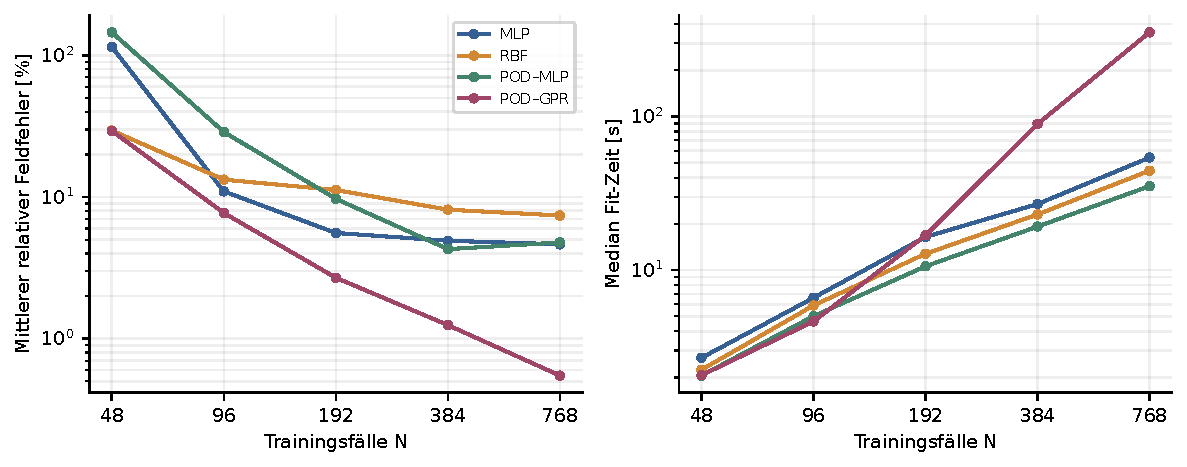
\includegraphics[width=\textwidth]{lernkurven.pdf}\caption{Mittlerer Interpolationsfeldfehler und mediane öffentliche Fit-Zeit gegen die Trainingsgröße. Logarithmische Achsen. Die Konfigurationen wurden bei $N=384$ festgelegt; die Art der Wiederholung ändert sich beim Vollpool. Eigene Darstellung.}\label{fig:lernkurven}\end{figure}

Die Fit-Zeit des ausgewerteten POD--GPR-Hauptmodells beträgt 353,5687942\,s. Zwei weitere Fits derselben Konfiguration dauern 337,1902846\,s und 336,1487963\,s. Der Median dieser drei vergleichbaren Zeitmessungen beträgt 337,1902846\,s; Trainingsfälle, Konfiguration und Fingerprints stimmen überein. Der Median ist somit nicht die Fit-Zeit des einzelnen ausgewerteten Hauptmodells. Die Zeiten umfassen den öffentlichen Fit, aber weder Speichern noch Validierungsvorhersage. Die Fit-Zeiten der neuronalen Seed-42-Hauptmodelle betragen 52,67\,s, 43,71\,s und 32,26\,s für MLP, RBF und POD--MLP.

\section{Einfluss der Trainingsverteilung}
Abbildung~\ref{fig:verteilung} zeigt bei $N=192$ den separaten Vergleich einer raumfüllenden und einer auf kleine Längen konzentrierten Auswahl. Die raumfüllende Auswahl erreicht für alle vier untersuchten Familien den geringeren mittleren Interpolationsfehler. Beispielsweise ergeben sich für POD--GPR 2,90\,\% gegenüber 5,08\,\%. Gleiche äußere Parametergrenzen bedeuten somit nicht notwendig eine vergleichbare Abdeckung im Inneren. Es handelt sich um die konkret untersuchten Designs, nicht um eine allgemeine Aussage über jede mögliche Verteilung.
\begin{figure}[htbp]\centering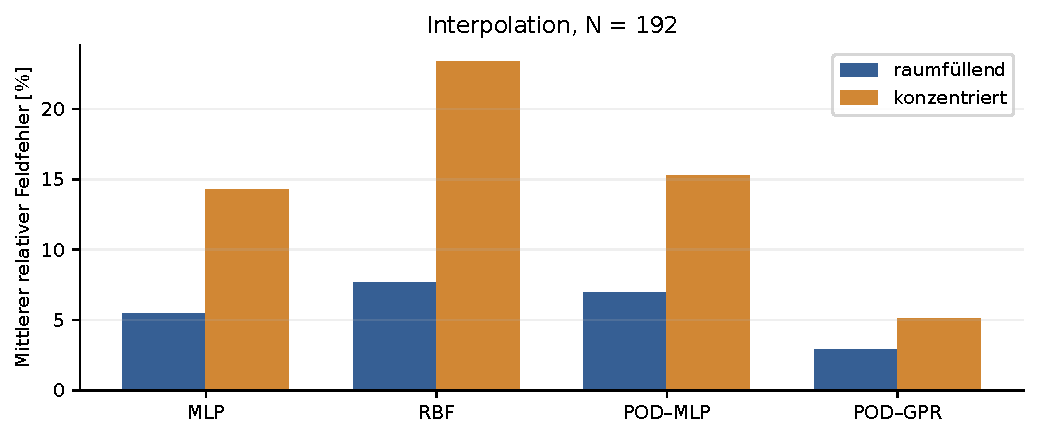
\includegraphics[width=.86\textwidth]{verteilung.pdf}\caption{Einfluss der Trainingsverteilung bei $N=192$ auf dieselben Interpolationsfälle. Eigene Darstellung der separaten Verteilungsstudie.}\label{fig:verteilung}\end{figure}

\section{POD-Rang, Fehleranteile und Aufbauaufwand}
Abbildung~\ref{fig:pod} zeigt den Projektions- und Koeffizientenregressionsanteil sowie die geschätzte eigenständige Fit-Zeit für die drei Ränge im kontrollierten Vollpoolvergleich. Beide Methoden verwenden dieselbe Basis pro Rang. Es handelt sich je Methode und Rang um einen Lauf, nicht um ein Mittel über neuronale Initialisierungen. Für POD--GPR beträgt der vollständige Interpolationsfehler bei Rang 2 beziehungsweise 15 0,560\,\% beziehungsweise 0,549\,\%; die entsprechenden eigenständigen Fit-Schätzungen sind 70,53\,s und 348,22\,s. Für die Extrapolation ergeben sich 3,861\,\% und 3,854\,\%. Die Unterschiede sind deskriptiv und nach Testeinsicht ermittelt.
\begin{figure}[htbp]\centering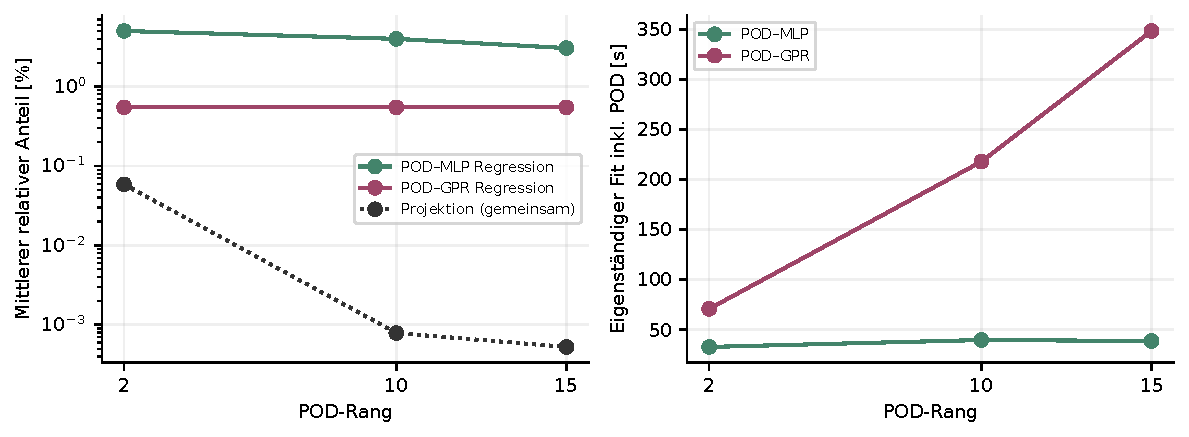
\includegraphics[width=\textwidth]{pod_rang.pdf}\caption{Kontrollierter POD-Vollpoolvergleich: mittlere relative Projektions- und Regressionsanteile für Interpolation sowie eigenständiger Fit einschließlich separat gemessener POD-Kosten. Ein Lauf je Rang und Methode; logarithmische Fehlerachse. Eigene Darstellung.}\label{fig:pod}\end{figure}

\section{Extrapolationsausreißer}
Der größte beobachtete relative Vollpoolfehler aller vier Familien betrifft Fall 830644. Der extrapolierte Parameter ist $F_z=-29{,}9502$\,N, oberhalb der Trainingsgrenze $-100$\,N und um 7,7833\,\% der Trainingsintervallbreite entfernt. Die Referenznorm beträgt $5{,}076\cdot10^{-7}$\,m. Der größte relative Fehler je Familie beträgt 638,23\,\% für MLP, 1253,55\,\% für RBF, 286,56\,\% für POD--MLP und 88,55\,\% für POD--GPR. Die Maxima von MLP und RBF stammen von anderen Initialisierungen als Seed 42.

Abbildung~\ref{fig:ausreisser} vergleicht für denselben Fall die vorab festgelegten Seed-42-Hauptmodelle. Die FEM-Spitze liegt bei $-0{,}001033$\,mm. Die direkte MLP-, RBF- und POD--MLP-Vorhersage besitzen dort ein falsches positives Vorzeichen; POD--GPR sagt $-0{,}001955$\,mm vorher. Die jeweiligen absoluten Feldfehler sind ungleich null. Unter den 13 größten relativen Fehlern je Seed-42-Modell liegen sieben, neun, sechs beziehungsweise acht Fälle in der zehn Fälle umfassenden Gruppe $F_z$ oberhalb der Grenze. Der Median der Referenznorm über alle 128 Extrapolationsfälle beträgt $5{,}04\cdot10^{-5}$\,m und ist damit deutlich größer als die typischen Normen der größten relativen Fehler. Niedrige Referenznormen verstärken die relative Kennzahl; sie erklären jedoch nicht alle absoluten Feldabweichungen.
\begin{figure}[htbp]\centering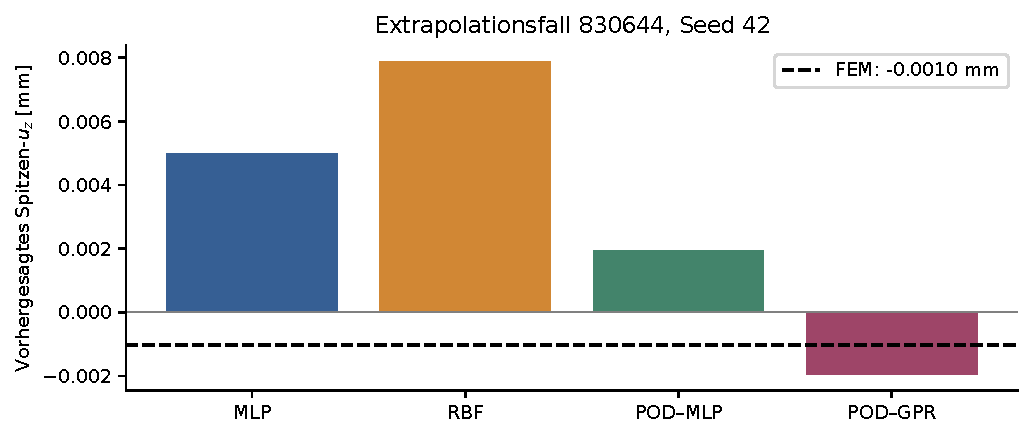
\includegraphics[width=.85\textwidth]{ausreisser.pdf}\caption{Vorhergesagtes vorzeichenbehaftetes Spitzen-$u_z$ des Extrapolationsfalls 830644 für die Seed-42-Hauptmodelle. Die gestrichelte Linie zeigt die FEM-Referenz. Eigene Darstellung.}\label{fig:ausreisser}\end{figure}

\section{Zusätzlicher FEM- und Vorhersagebenchmark}
Der nachträgliche Benchmark verwendet zwölf vorab unabhängig vom Fehler gewählte Interpolationsfälle auf einem AMD Ryzen 5 4500U unter MATLAB R2025b. Nach einem FEM-Warm-up werden die Fälle je zweimal seriell gelöst, im zweiten Durchlauf in umgekehrter Reihenfolge. Der FEM-Aufruf umfasst Geometrie, Netz, Lösung, vollständige Feldinterpolation sowie Spitzenabfrage und Prüfungen. Für die eingefrorenen Seed-42-Modelle werden nach Warm-up 30 vollständige Einzelfallaufrufe pro Fall und 30 gemeinsame 12er-Batches gemessen. Das Laden wird getrennt erfasst; Dateizugriffe sind aus den eigentlichen Vorhersagezeiten ausgeschlossen.

Der Median der fallweisen FEM-Mediane beträgt 2,189\,s; der Interquartilsabstand zwischen Fällen beträgt 1,734\,s. Die Summe der zwölf fallweisen FEM-Mediane ist 29,418\,s und keine Messung eines optimierten FEM-Batchsolvers. Abbildung~\ref{fig:zeiten} zeigt die Surrogatzeiten. Beim Einzelfall liegen sie zwischen 7,573 und 9,252\,ms; beim gemeinsamen 12er-Aufruf zwischen 9,835 und 18,469\,ms. FEM enthält zusätzliche Spitzenabfragen und Prüfungen; die Messumfänge sind deshalb nicht völlig identisch.
\begin{figure}[htbp]\centering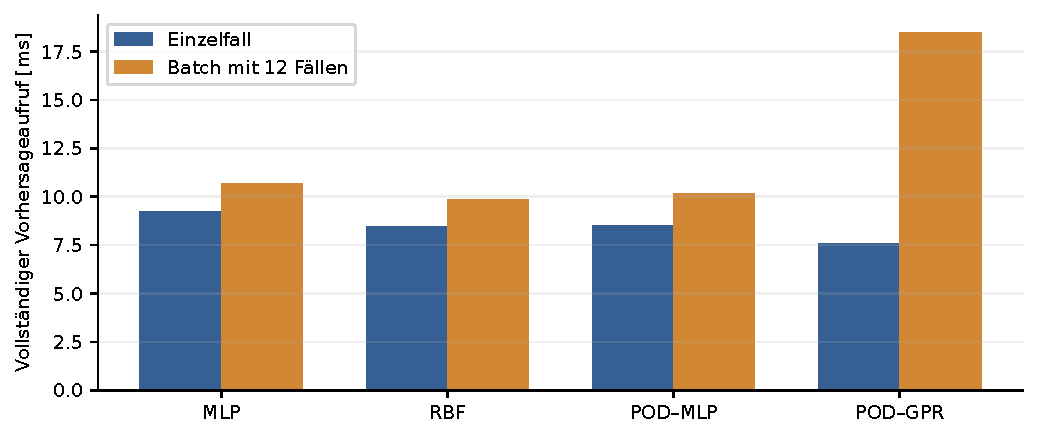
\includegraphics[width=.85\textwidth]{vorhersagezeit.pdf}\caption{Median vollständiger Surrogataufrufe im nachträglichen Benchmark: ein Fall und gemeinsamer 12er-Batch. Ladezeiten sind ausgeschlossen. Eigene Darstellung.}\label{fig:zeiten}\end{figure}

\section{Bedingte Amortisationsszenarien}
Für einen positiven Zeitgewinn pro Einzelfall wird die rechnerische Schwelle bestimmt durch
\begin{equation}
 Q_{\mathrm{BE}}=\left\lceil\frac{C_{\mathrm{offline}}}{t_{\mathrm{FEM}}-t_{\mathrm{Surrogat}}}\right\rceil.
\end{equation}
Mit vorhandenen Trainings- und Validierungsdaten umfasst $C_{\mathrm{offline}}$ hier den Fit des Seed-42-Hauptmodells, wahlweise zuzüglich äußerer Familiensuche. Für POD--GPR ergeben sich 163 Einzelfälle mit Fit beziehungsweise 714 mit Fit und Suche. Im seriellen FEM-/12er-Batch-Szenario sind es 156 beziehungsweise 636 Fälle. Fit und Suche stammen aus der Hauptstudie, Vorhersage- und FEM-Zeiten aus dem späteren Benchmark auf derselben Maschine. Die Werte sind bedingte Szenarien auf Medianbasis, ohne Unsicherheitsintervall und ohne Lade-, Speicher- oder Qualitätssicherungskosten.

Für eine hypothetische Neuerzeugung wird lediglich eine gemischte historische Rechenannahme aus 1632,92\,s Trainings-Solverzeit und 566,11\,s aktiver Validierungserzeugung angesetzt. Die Trainings-Gesamtzeit fehlt; diese Summe ist keine neu kontrolliert gemessene vollständige Datenerzeugung. Testdatenerzeugung, Pilot und weitere Studienkosten bleiben in den Szenarien unberücksichtigt. Die vollständigen methodenspezifischen Zahlen und Kostenabgrenzungen stehen im Anhang.
